%% If you have any problems using this template, please contact the author: %%
%% Chris Carmona: carmona@stats.ox.ac.uk ; chriscarmona.me %%

\documentclass{beamer}

\usepackage{mathrsfs,amsmath}

%load any additional packages

\usepackage[UKenglish]{babel}
\usepackage[utf8]{inputenc} % so we can input characters with accents (e.g. ő)

\usepackage{statsbeamer}

\usepackage{graphicx} % ease graphics management

\usefonttheme{serif} % change font to allow \textbf{}
\usepackage{charter} % Nicer fonts

\usepackage{amsmath,amsthm,amssymb} % for math equations

\usepackage{natbib} % richer citation
\usepackage{breakcites} % avoid overfull hbox for long cites

\graphicspath{{images/}{../python/figs/}}  % define folder with images
%% Information (author, title, etc.) %%

\title[Condition monitoring]{% short title for footer
    Introduction to condition monitoring of roller bearings
    \vspace{0.5cm}
}

\author{ Geir Kulia}

% \institute{
%         \textit{Department of Statistics}\\
%         \textit{University of Oxford}
%         \vspace{0.5cm}
% }
\date[UiA 27.10.21]{% short date for footer
    University of Agder\\27 October 2021
}


%% Content of slides %%
%%%%%%%%%%%%%%%%%%%%
\begin{document}
%%%%%%%%%%%%%%%%%%%%

% Title slide %
{
    \setbeamertemplate{footline}{}
    \setbeamertemplate{headline}{}
    \setbeamercolor{background canvas}{bg=oxfordblue}
    \maketitle
}

% \input{slides/table-of-contents}

%now include the slides
\setbeamercovered{transparent}

%----------------------------%
% Contents slide

%----------------------------%


%----------------------------%
\begin{frame}
    \frametitle{Motivation}
    \small
\begin{columns}
\begin{column}{0.5\textwidth}
    Rolling element bearings are widely used in rotating machines. Their failure is one of the most frequent reasons for machine breakdown. 
    \\[1\baselineskip]
    This keynote will show the calculation of an elementary envelope spectrum to identify faults by monitoring for abnormalities in a bearing's
    \begin{itemize}
        \item Outer race
        \item Inner race 
        \item Fundamental train
        \item Rolling elements
    \end{itemize}
\end{column}
\begin{column}{0.5\textwidth}  %%<--- here
    \begin{figure}
        \centering
        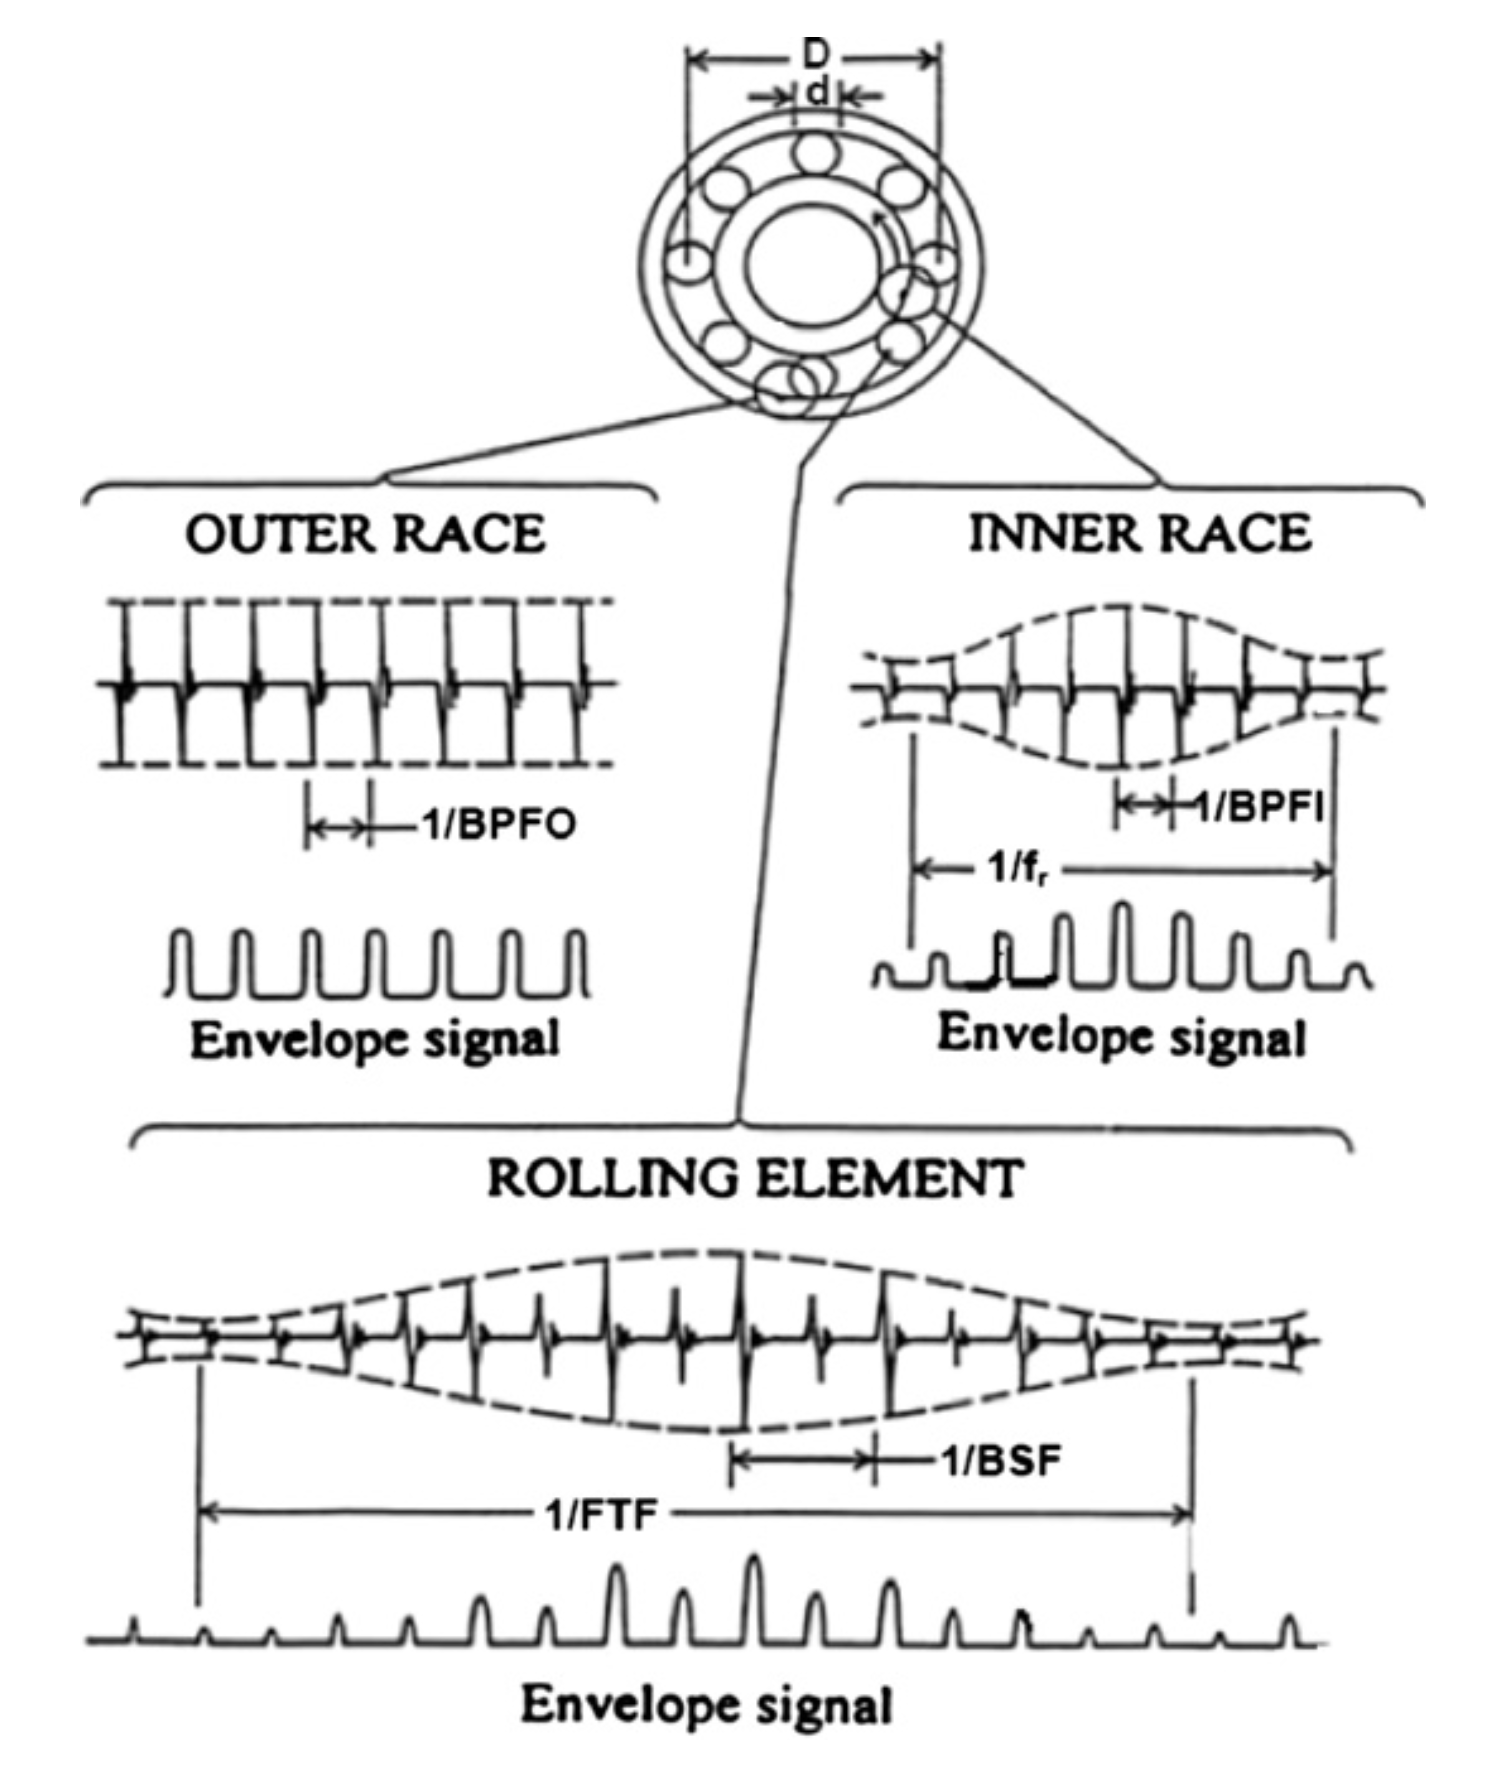
\includegraphics[width=\textwidth]{images/bearing.png}
        \caption{Typical signals and envelope signals from local faults in rolling element bearings. \cite{cm}.}
        \label{fig:spectrum}
    \end{figure}
\end{column}
\end{columns}
\end{frame}

\begin{frame}
    \frametitle{Measurement}
    \small
    A high density accelerometer is used to monitor the roller bearing.  The accelerometer can be either permanently mounted or a portable device.
    \begin{figure}
        \centering
        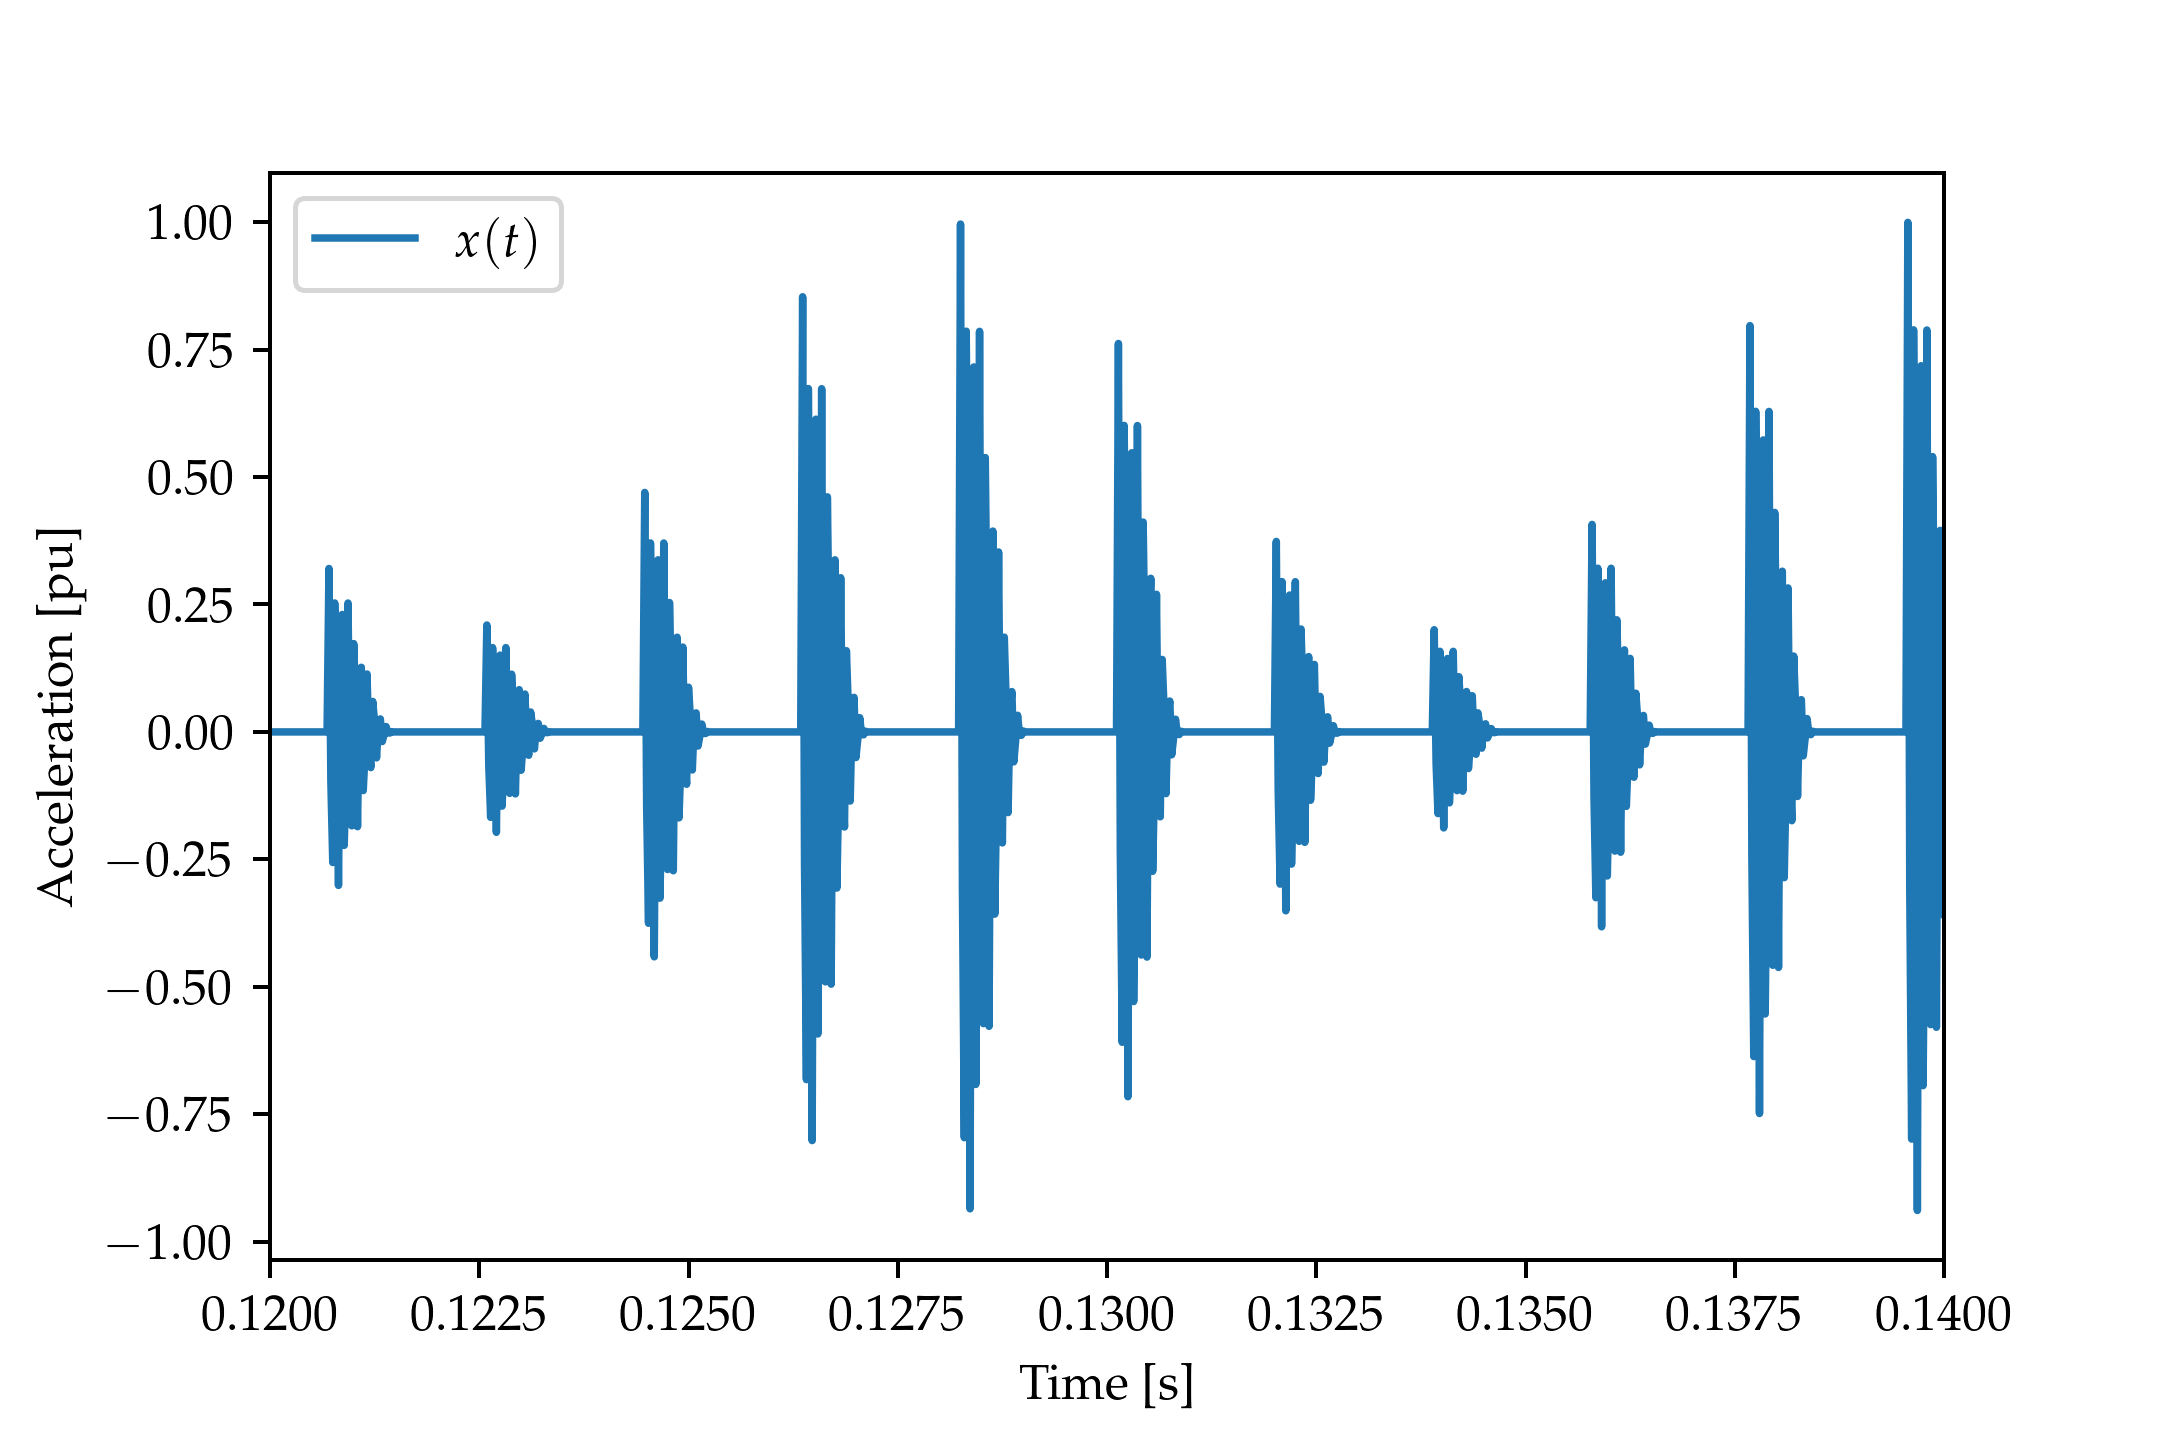
\includegraphics[width=0.5\textwidth]{raw.png}
        \caption{Example of a fingerprint of a damaged roller bearing.}
        \label{fig:raw}
    \end{figure}
    The sampling rate, $f_s$ is usually around $f_s \in [50\text{ kHz}, 100\text{ kHz}]$.
   
\end{frame}
\begin{frame}
    \frametitle{The analytic signal}
    \small
    The acceleration signal is high-pass filtered to remove unwanted machine noise.  The design of these filters are outside the scope of this presentation.  The resulting acceleration signal $x(t)$ is then used to generate an analytic signal, $z(t)$.  It is defined as 
    \begin{equation}
        z(t) = x(t) + j y(t) = a(t) e^{j\theta}
    \end{equation}
    
    where $j^2=-1$ and $y(t)$ is the Hilbert transform of $x(t)$ can conceptually be considered as the convolution $x(t) * \frac{1}{t}$. and where the amplitude is
    
    \begin{equation}
        a(t) = \mid{z(t)}\mid = \sqrt{x^2(t)+y^2(t)}
    \end{equation}
    
    and the phase (not to be confused with phase shift) is
    
    \begin{equation}
        \theta(t) = \angle{z(t)} = \arctan\Big(\frac{y}{x}\Big)
    \end{equation}
   
\end{frame}
\begin{frame}
    \frametitle{The analytic signal}
    \small
    
    \begin{figure}
        \centering
        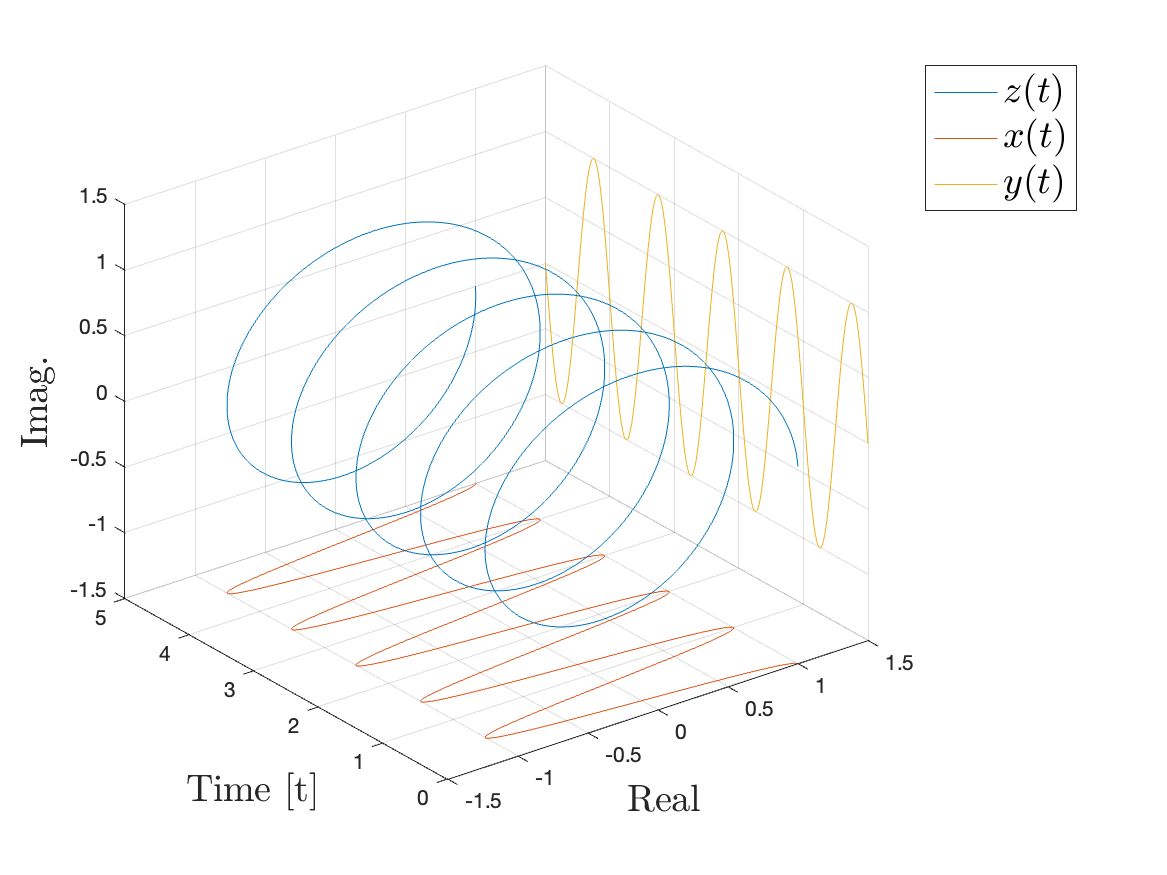
\includegraphics[width=0.75\textwidth]{images/analytic-signal.png}
        \caption{Analytic signal $z(t)$ of a real signal $x(t)=\cos(2\pi t)$, so that $z(t)=\cos(2\pi t) + j\sin(2\pi t) = 1 e^{j2\pi t}$}
        \label{fig:spectrum}
    \end{figure}
   
\end{frame}

\begin{frame}
    \frametitle{The envelope spectrum}
    \small
    
    Using the analytic signal
    \begin{equation}
        z(t)=x(t)+jy(t) = a(t) e^{j\theta}
    \end{equation}
    
    we can define the envelope as
    
    \begin{equation}
       e(t) = |z(t)| = | x(t) + jy(t) | = a(t)
    \end{equation}
   
   The envelope spectrum is thus defined as the fourier spectrum of the envelope, $a(t)$
   
   \begin{equation}
       E_{f}(\omega) = \mathscr{F}\{a(t)\} = \int_{-\infty}^{\infty} e(t) e^{-j\omega t} dt
   \end{equation}
   
   A envelope periodogram is then defined as 
   
   \begin{equation}
       E(\omega) = |E_{f}(\omega)|^2
   \end{equation}
   
\end{frame}
\begin{frame}
    \frametitle{The envelope of a signal}
    \small
    
    \begin{figure}
        \centering
        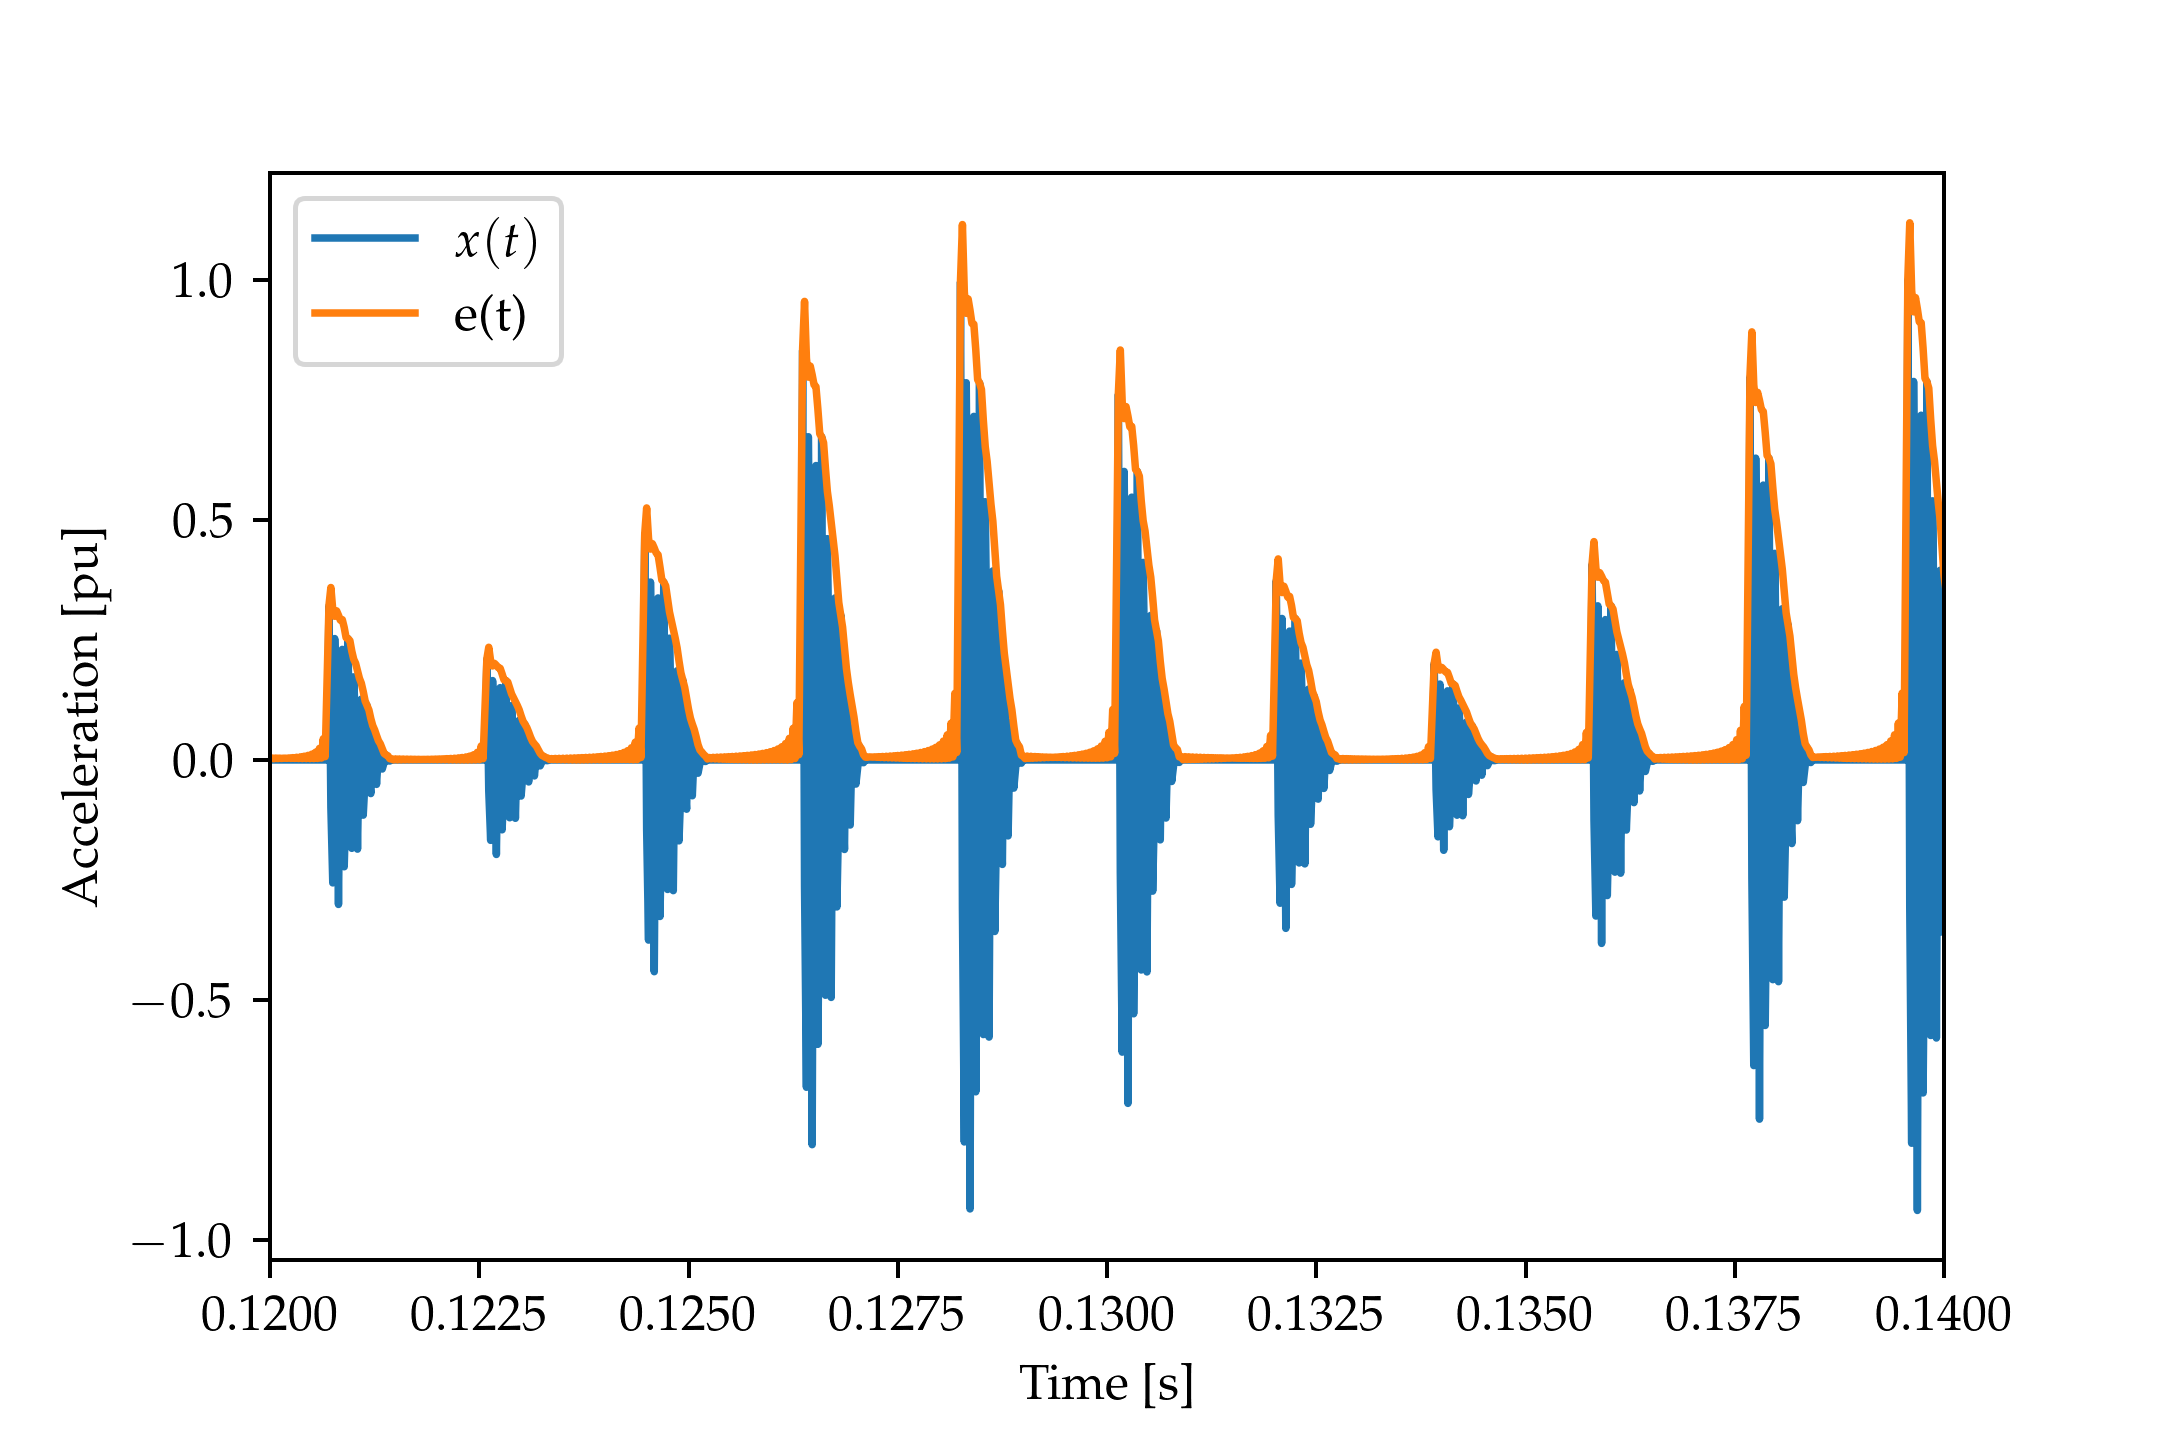
\includegraphics[width=0.75\textwidth]{images/raw_w_envelope.png}
        \caption{Example of a fingerprint of a damaged roller bearing with its envelope}
        \label{fig:spectrum}
    \end{figure}
   
\end{frame}
\begin{frame}
    \frametitle{Order spectrum}
    \small
    
    In the envelope spectrum, $E(\omega)$, the frequencies will scale with the shaft speed, $f_r$. The order spectrum is an envelope spectrum where the frequencies are normalized with the rotation speed, denoted as order, so that
    
    \begin{equation}
        [\text{order}] = \Big[\frac{f}{f_r}\Big]
    \end{equation}
    
    where in the order domain one get that $1 = f_r$.   
\end{frame}
\begin{frame}
    \frametitle{The envelope and order spectrum}
    \small
    
    \begin{figure}
        \centering
        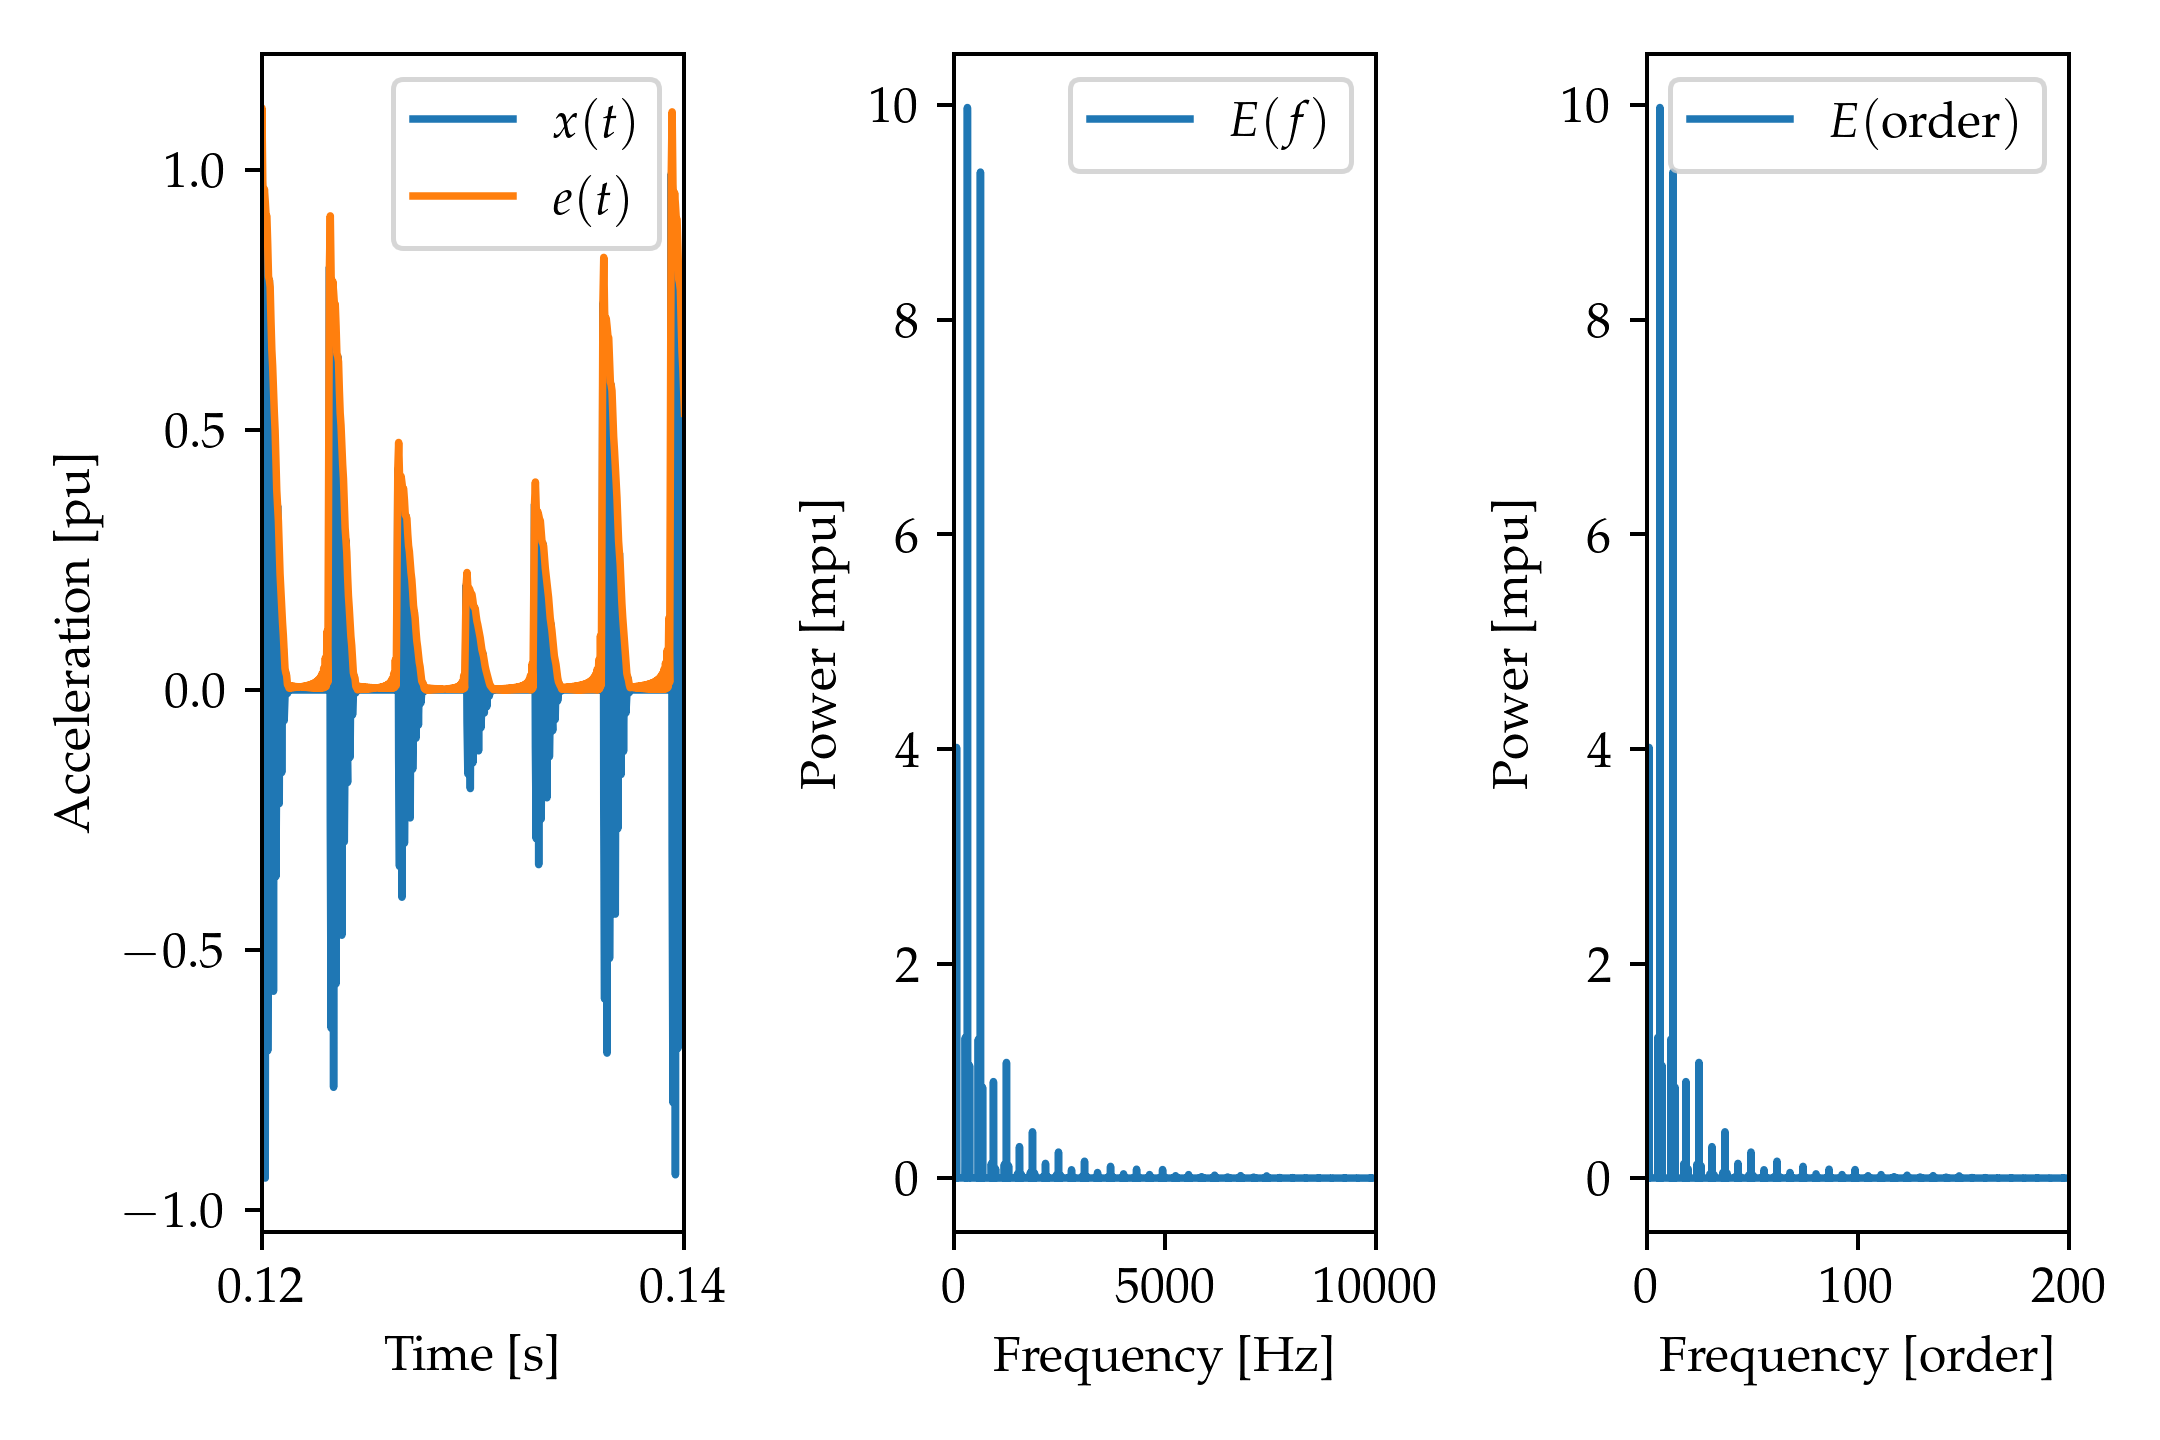
\includegraphics[width=0.75\textwidth]{order_spectrum.png}
        \caption{Example of a fingerprint of a damaged roller bearing $x(t)$ with its envelope $e(t)$, its envelope spectrum $E(f)$ and its order spectrum $E($order$)$}
        \label{fig:order_spectrum}
    \end{figure}
   
\end{frame}
%----------------------------%


%----------------------------%
% Conclusions

% {\usebackgroundtemplate{%
%   
\includegraphics[width=\paperwidth,height=\paperheight]{images/logo}} 
\begin{frame}
    \frametitle{}
    \centering
    
    % \Large\color{oxfordblue}
    Thank you!

    \vspace{0.5cm}
    geir@sal.no
    
    \vspace{0.5cm}
    
    Give anonymous feedback on
    https://www.admonymous.co/geir
    
    \vspace{0.5cm}
    Find the presentation and code at
    https://github.com/kulia/uia-cm-2021-10-26

\end{frame}
% }
%----------------------------%

% References slide
\begin{frame}
\frametitle{References}
\small
\bibliographystyle{plain}
\bibliography{references} % bibliography file
\end{frame}

% Appendices

\begin{frame}
    \frametitle{The Hilbert Transform}
    \small
    The analytic signal is defined as 
    \begin{equation}
        z(t) = x(t) + j y(t) = a(t) e^{j\theta}
    \end{equation}
    
    where $j^2=-1$ and $y(t)$ is the Hilbert transform of $x(t)$ so that
    
    \begin{equation}
        y(t) = \frac{\rm{pv}}{\pi} \int_{-\infty}^{\infty} \frac{x(\tau)}{t-\tau} d\tau
    \end{equation}
    
    where pv denotes the Cauchy principal value.  The Hilbert transform can conceptually be considered as the convolution $x(t) * \frac{1}{t}$.
   
\end{frame}

%%%%%%%%%%%%%%%%%%%%
\end{document}
%%%%%%%%%%%%%%%%%%%%
